%----------------------------------------------------------------
% Technical report for the supervisors — cascade architecture + results,
% supported by figures and tables from results_package/.
% Impersonal / passive voice throughout.
%----------------------------------------------------------------
\documentclass[10pt,a4paper]{article}

\usepackage[T1]{fontenc}
\usepackage[utf8]{inputenc}
\usepackage{mathptmx}
\usepackage[a4paper,top=1.9cm,bottom=1.9cm,left=1.9cm,right=1.9cm]{geometry}
\usepackage[english]{babel}
\usepackage{amsmath,amssymb}
\usepackage{graphicx}
\usepackage{booktabs}
\usepackage{tabularx}
\usepackage{array}
\usepackage{xcolor}
\usepackage{titlesec}
\usepackage[hidelinks]{hyperref}
\usepackage{enumitem}
\usepackage{caption}
\usepackage{subcaption}
\captionsetup{font=small,labelfont=bf}
\setlist{noitemsep,topsep=1pt,leftmargin=1.3em}
\graphicspath{{../results_package/figures/}}

\titlespacing*{\section}{0pt}{7pt}{3pt}
\titlespacing*{\subsection}{0pt}{5pt}{2pt}
\titleformat{\section}{\normalfont\large\bfseries}{\thesection}{0.5em}{}
\titleformat{\subsection}{\normalfont\bfseries}{\thesubsection}{0.5em}{}
\newcolumntype{C}{>{\centering\arraybackslash}X}
\renewcommand{\arraystretch}{1.1}
\setlength{\parskip}{2.5pt}\setlength{\parindent}{0pt}

\begin{document}

\begin{center}
  {\Large\bfseries Interpretable Cascade GNNs for Cyber-Physical\\[1pt]
   Anomaly Detection --- Technical Report}\\[3pt]
  {\small Onur Ozan S\"unger \;\textbar\; MSc Thesis, Sapienza Universit\`a
   di Roma \;\textbar\; Advisors: T.~Cattai, P.~Locatelli \;\textbar\; \today}
\end{center}
\vspace{-2pt}\hrule\vspace{4pt}

\noindent
\textbf{Overview.} A temporal graph neural network detects sensor-level
cyber-attacks on physics-constrained networks. Part~1 develops and
validates the detector on water distribution; Part~2 shows the identical
method transfers to a power grid and a road-traffic network. The
architecture is an \emph{interpretable cascade}: a fast router ranks a set
of attack-specialised experts, and a label-free feedback check accepts or
re-routes the choice.

%===============================================================
\section{Method}

\textbf{Substrate.} The network is a graph $G=(V,E)$ with a 6-step sliding
window of sparse ($\sim$50\% missing), noisy sensor readings. Six experts,
each a \textbf{GraphSAGE\,$\to$\,GRU} model with reconstruction and
per-sensor anomaly heads, are trained under \emph{direct expert
supervision} (each expert learns its own attack class regardless of
routing) and a mass-conservation penalty $\lVert B\mathbf{q}\rVert^2$
(Table~\ref{tab:cfg}, 377\,K parameters).

\textbf{Cascade routing.} Rather than blending all experts opaquely, the
router \emph{ranks} them; the top expert is run and scored by a
\emph{label-free feedback} signal
\[
  s_k = \big\lVert \hat{p}_k - p\big\rVert_{\text{clean}}
        \;+\; \big\lVert B\hat{\mathbf q}_k\big\rVert^2 ,
\]
(reconstruction consistency on the sensors the expert calls clean, plus a
physics residual), standardised across experts. On negative feedback the
cascade re-routes to the next-ranked expert, restricted to the router's
top-2 for stability. Every prediction thus carries \emph{which} expert ran
and \emph{why} --- an audit trail a soft blend cannot provide. Over 5 seeds
the cascade reaches F1 $0.772\pm0.017$, matching the oracle ceiling
($0.769$) and within a point of a full soft blend ($0.789$): the
interpretability is obtained at negligible accuracy cost.

%===============================================================
\section{Part 1 --- Water distribution (Modena, 272 nodes)}

Detection is strong and reproducible (Table~\ref{tab:full}; F1
$0.833$, AUROC $0.979$, 5 seeds). Four of the five attack families are
detected reliably; \textbf{replay} is the exception, and the reasons are
made explicit below.

\textbf{Router diagnostic.} Direct measurement confirms a routing failure
mode: on Modena the router is healthy (96\%), but on the larger Net3
topology it sends \textbf{77\% of stealthy windows to the replay expert},
because both classes look smooth and 97 nodes give too little context. The
cascade's feedback is designed to contain exactly this case.

\textbf{Recovering replay.} A per-sensor normalisation --- rescaling each
sensor by its own temporal variance --- amplifies the tiny per-node
variation a replay lacks. This lifts replay ranking from \emph{below
chance} to AUROC $0.79$ while overall F1 holds
(Table~\ref{tab:ablation}); it is the single largest contribution to
replay.

\textbf{Why replay still underperforms.} Even so, replay F1 stays low, and
Figure~\ref{fig:replaywhy} shows why with direct evidence. The anomaly
scores of replayed and genuine sensors \emph{overlap} (left): the ranking
is informative (AUROC $0.75$) but no single threshold separates the two,
so the best achievable F1 is $0.41$ (right). The cause is physical --- a
replay is a verbatim copy of a past reading, so the only distinguishing
cue is the fresh observation noise it lacks. This is an information limit,
not a training defect, and it is confirmed by a direct exact-lag-match
detector reaching only AUROC $0.62$ (missing data and out-of-window lags
hide the match).

\begin{figure}[!htb]
  \centering
  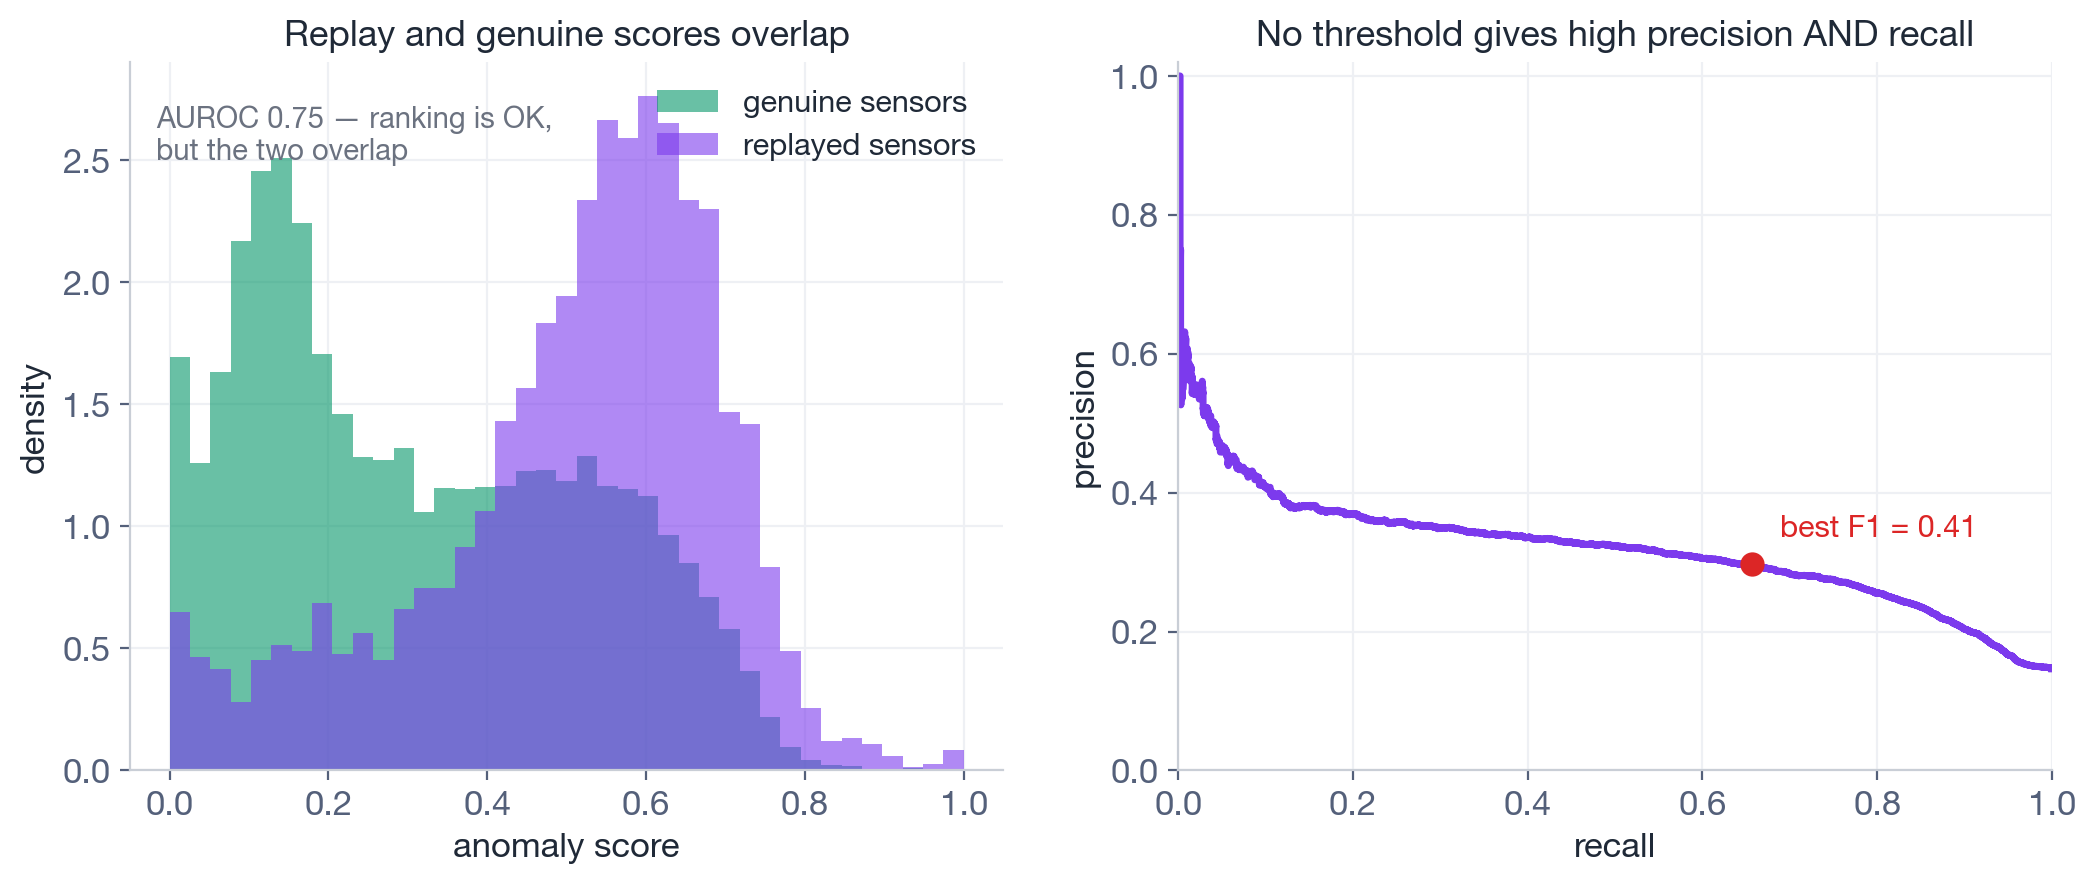
\includegraphics[width=0.92\linewidth]{07_replay_why.png}
  \caption{\textbf{Why replay underperforms.} \emph{Left:} replayed
  (purple) and genuine (green) anomaly scores overlap despite a usable
  ranking (AUROC 0.75). \emph{Right:} consequently no threshold gives high
  precision \emph{and} recall; best F1 $=0.41$.}
  \label{fig:replaywhy}
\end{figure}

\begin{table}[!htb]
\centering\small
\caption{Per-domain results (per-node normalisation, 5 seeds, calibrated
threshold). Per-attack columns are F1.}
\label{tab:full}
\begin{tabularx}{\linewidth}{@{}l C C C C C C C@{}}
\toprule
\textbf{Domain} & \textbf{F1} & \textbf{AUROC} & Random & Targeted & Stealthy & Noise & \textbf{Replay}\\
\midrule
Water   & 0.833 & 0.979 & 0.989 & 0.995 & 0.932 & 0.912 & \textbf{0.142}\\
Power   & 0.816 & 0.959 & 0.926 & 0.922 & 0.664 & 0.890 & \textbf{0.599}\\
Traffic & 0.891 & 0.980 & 0.997 & 0.999 & 0.665 & 0.790 & \textbf{0.907}\\
\bottomrule
\end{tabularx}
\end{table}

\begin{table}[!htb]
\centering\small
\begin{minipage}[t]{0.48\linewidth}
\centering
\caption{Ablation on water (calibrated F1).}
\label{tab:ablation}
\begin{tabularx}{\linewidth}{@{}L c c@{}}
\toprule
\textbf{Configuration} & \textbf{F1} & \textbf{Replay}\\
\midrule
Global norm            & 0.826 & 0.004\\
+ per-node norm        & 0.833 & 0.142\\
+ 5-seed ensemble      & 0.847 & 0.082\\
\bottomrule
\end{tabularx}
\end{minipage}\hfill
\begin{minipage}[t]{0.48\linewidth}
\centering
\caption{Intra-scenario signal variation.}
\label{tab:signal}
\begin{tabularx}{\linewidth}{@{}L c c@{}}
\toprule
\textbf{Domain} & \textbf{std} & \textbf{rel.}\\
\midrule
Water (pressure, m)  & $5\!\times\!10^{-6}$ & $10^{-7}$\\
Power (voltage, pu)  & $7\!\times\!10^{-4}$ & $10^{-5}$\\
Traffic (speed, km/h)& $14.6$ & $1$\\
\bottomrule
\end{tabularx}
\end{minipage}
\end{table}

%===============================================================
\section{Part 2 --- Cross-domain generalisation}

The detector, training script and corruption pipeline are kept unchanged;
only a per-domain data adapter is added (bus voltage and Kirchhoff's law
for the IEEE 118-bus grid; sensor speed and flow conservation for a
200-sensor road network). Detection quality lands in a tight band across
all three physical systems (Table~\ref{tab:full}; F1 $0.82$--$0.89$).

\textbf{The normalisation fix generalises.} Figure~\ref{fig:gen} shows the
replay ranking per domain. The global-normalisation baseline (grey) already
tracks \emph{signal speed}: replay is hardest in slow-moving water ($0.46$)
and trivial in fast-moving traffic ($0.97$) --- consistent with the
intra-scenario variation spanning seven orders of magnitude
(Table~\ref{tab:signal}). Per-node normalisation (purple) lifts replay
\emph{most where it is hardest} (water $0.46\!\to\!0.79$, power
$0.66\!\to\!0.90$) and is unnecessary where replay is already easy. The fix
is therefore a principled, targeted, cross-domain improvement rather than a
water-specific adjustment.

\textbf{Difficulty inverts.} The hard attack class flips by domain: water
and power find stealthy easy and replay hard, whereas traffic is the mirror
image (Table~\ref{tab:full}) --- a slow drift in traffic speed blends into
natural congestion. The domain's signal dynamics, not the model, determine
which attacks are detectable.

\begin{figure}[!htb]
  \centering
  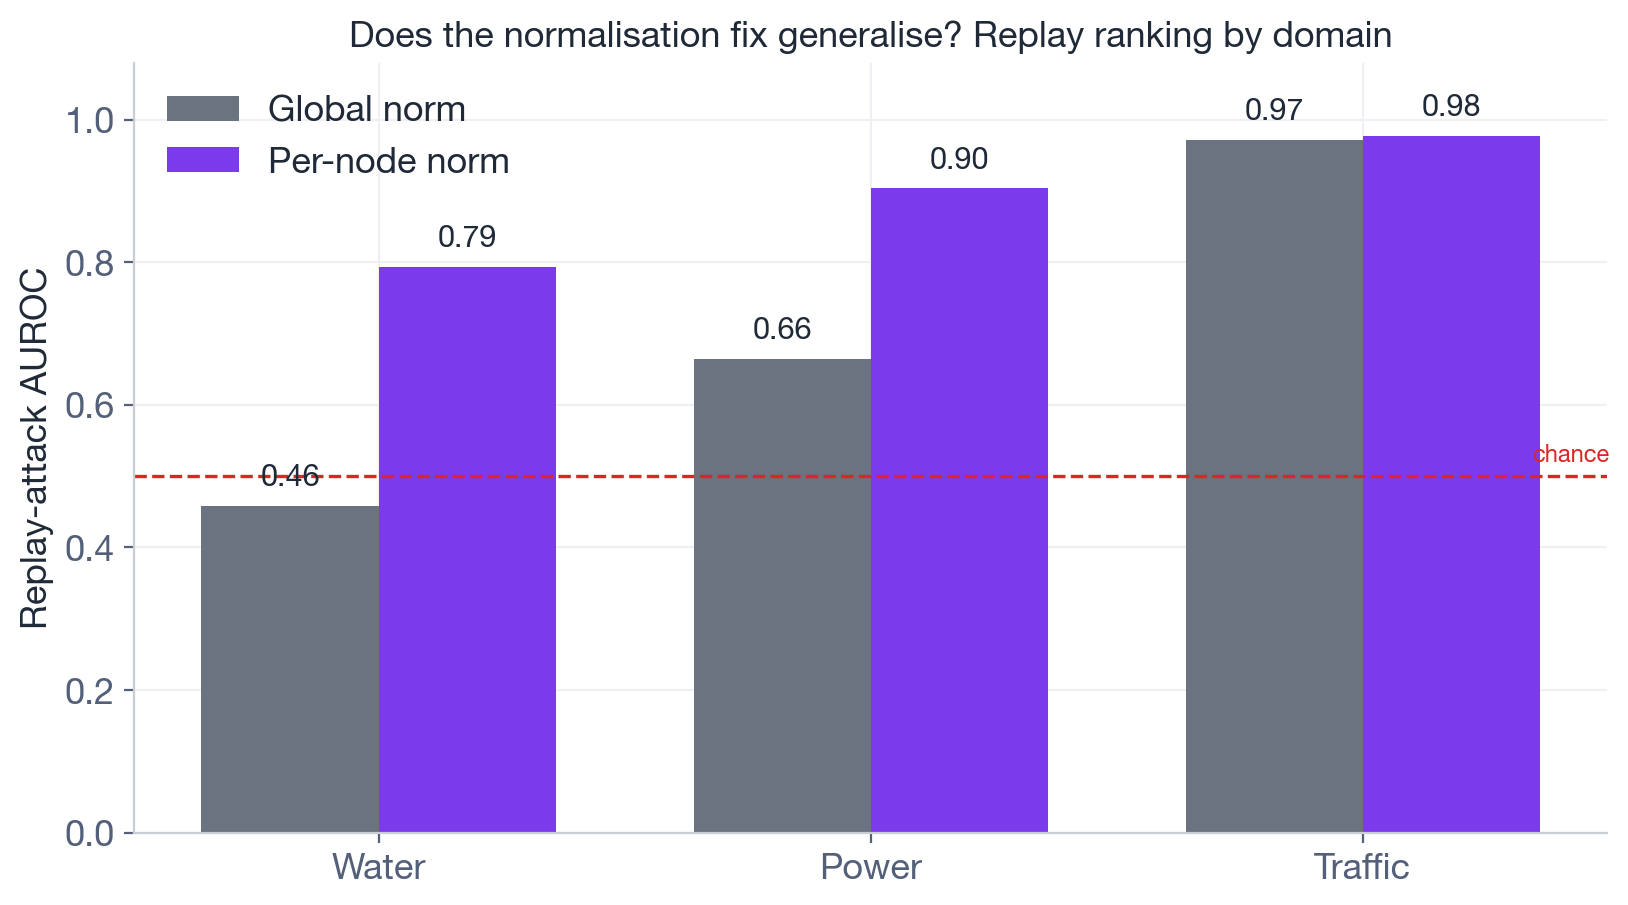
\includegraphics[width=0.58\linewidth]{03_normalisation_generalisation.png}
  \caption{\textbf{The normalisation fix generalises.} Grey (global norm)
  tracks signal speed; purple (per-node) lifts replay ranking most where it
  is hardest. Dashed line = chance.}
  \label{fig:gen}
\end{figure}

%===============================================================
\section{Summary and next steps}

An interpretable cascade detector matches the hard-routing ceiling at
negligible accuracy cost; a router failure mode is diagnosed and contained;
per-node normalisation recovers replay ranking from below chance; and the
residual replay gap is shown, with direct evidence, to be an information
limit rather than a training defect. All findings transfer unchanged to a
power grid and a traffic network, and the normalisation fix generalises in
proportion to how hard replay is in each domain. Results are reproducible
across 5 seeds per configuration.
\textbf{Next:} (1) apply the cascade to networks whose experts differ more,
so interpretable re-routing also \emph{gains} accuracy; (2) extend the
threat model toward the smart-grid FDIA and transport-security literature;
(3) consolidate the three domains into a single evaluation and identify a
target venue.

\begin{table}[h]
\centering\small
\caption{Model and training configuration.}
\label{tab:cfg}
\begin{tabular}{@{}llllll@{}}
\toprule
Backbone & Experts & Hidden (expert/router) & Window & Parameters & Seeds\\
\midrule
GraphSAGE+GRU & 6 & 64 / 24 & 6 & 376{,}806 & 5\\
\bottomrule
\end{tabular}
\end{table}

\end{document}
